\section{论文概览}

\subsection{核心问题}

Vision-Zero 讨论的是视觉语言模型（VLM）如何在没有人工问答标注、没有人工偏好反馈的情况下，通过多智能体自博弈获得可持续的后训练收益\cite{visionzero}。已有 VLM 强化学习方法大多仍依赖人工构造的问题、答案、推理轨迹或可验证奖励任务，这会带来两个瓶颈：一是多模态标注成本高，训练数据规模和多样性受限；二是模型能力上限容易被人工监督分布限定，很难主动发现超出既有监督样本的新策略。

论文的切入点是把 VLM 后训练改造成一个视觉版“谁是卧底”游戏。多个玩家参与同一局游戏，其中普通玩家看到原始图像，卧底看到空白图像或被修改过的图像。所有玩家先轮流给出一句视觉线索，然后普通玩家根据自己的图像和所有线索投票找出卧底。这个设置把视觉理解、语言表达、策略伪装、线索整合和不确定性判断放进同一个闭环，使模型在游戏中自动产生训练样本和奖励信号。

\subsection{一句话总结}

Vision-Zero 用“谁是卧底”式多智能体视觉自博弈，把任意无标签图像转化为可交互、可验证的训练环境，并通过 Iterative-SPO 在 clue-stage 自博弈和 decision-stage RLVR 之间切换，从而在零人工标注条件下提升 VLM 的推理、图表理解和视觉中心任务能力。

\subsection{与普通 RLVR 的区别}

普通 RLVR 往往需要预先设计问题、标准答案或规则化验证器。Vision-Zero 的关键不是直接为某个下游任务写奖励函数，而是构造一个可持续产生奖励的游戏环境：

\begin{itemize}
    \item 图像输入可以是任意无标签图像，训练不需要人工问答标注。
    \item 奖励来自游戏结果，例如卧底收到多少票、普通玩家是否投对卧底。
    \item 游戏难度随模型能力动态变化：卧底更会伪装时，普通玩家需要更强推理；普通玩家太容易识别卧底时，系统又切回线索阶段提高生成线索的博弈难度。
    \item 训练信号同时覆盖视觉观察、文本线索、跨轮对话和多角色策略，而不是只优化单轮问答正确率。
\end{itemize}

因此，Vision-Zero 可以看作是把“可验证奖励”从静态题库推进到交互式环境。奖励仍然可计算，但样本和难度来自多智能体互动，而不是人工写好的固定 QA。

\subsection{Figure 1：训练范式对比}

Figure~\ref{fig:visionzero-figure1} 对比了三类训练范式。监督学习依赖人工推理轨迹；传统强化学习虽然可以让模型学习推理过程，但通常仍依赖专家设计的问答对和验证奖励；Vision-Zero 则通过图像差异构造自博弈，让模型在游戏中持续生成训练数据。

\begin{figure}[H]
    \centering
    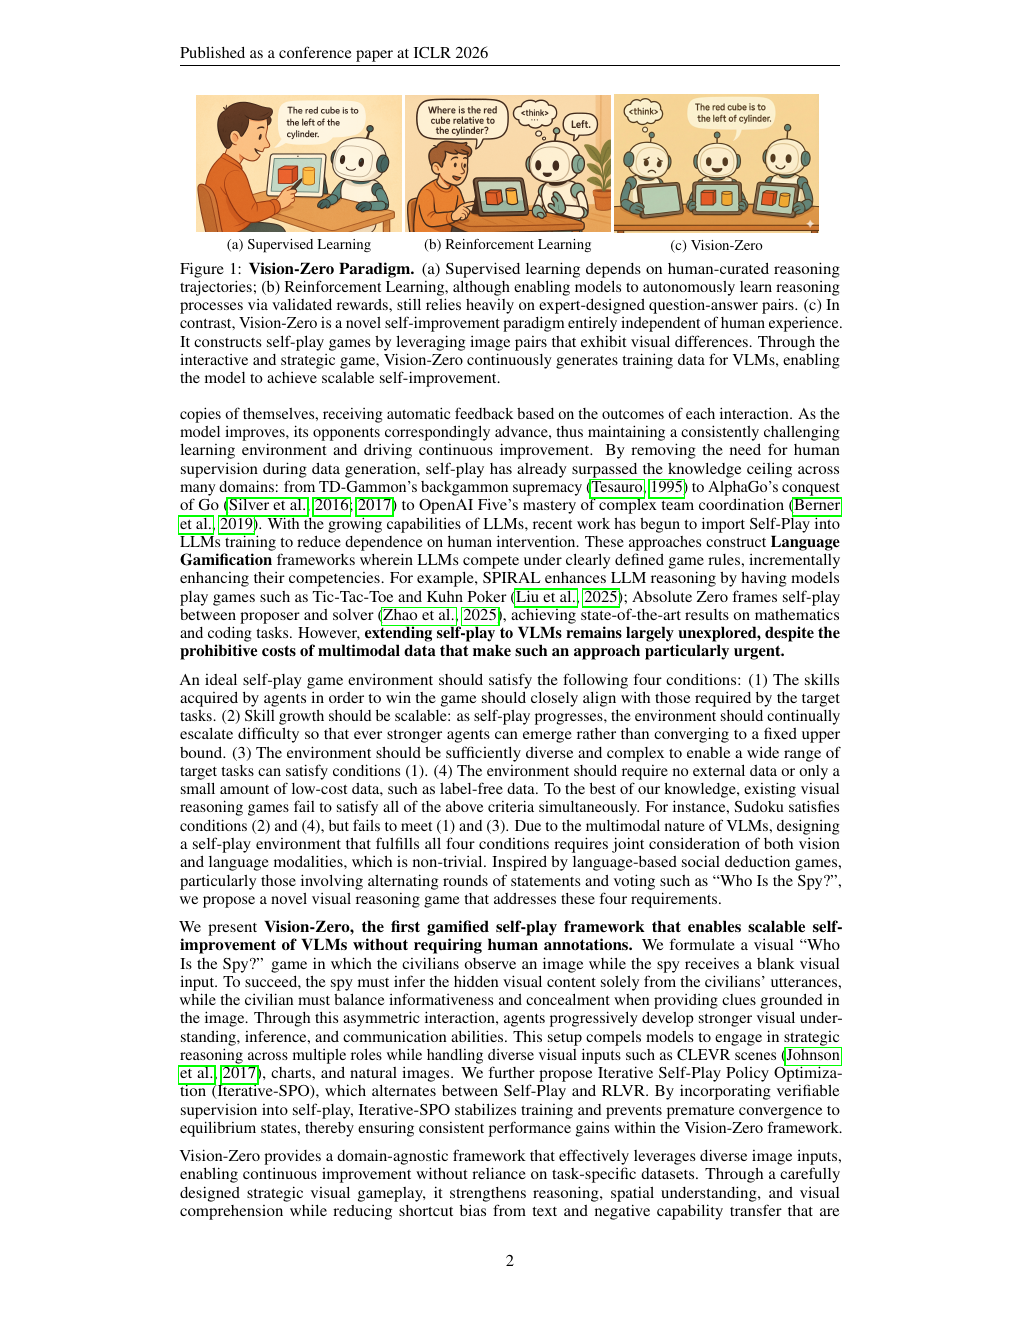
\includegraphics[width=0.95\textwidth]{figures/figure1_page.png}
    \caption{Vision-Zero 与监督学习、传统 RLVR 的范式对比。}
    \label{fig:visionzero-figure1}
\end{figure}

这张图背后的核心思想是：如果训练数据的产生也可以被游戏规则驱动，那么 VLM 后训练就不必始终围绕人工题库展开。模型能力提升后，游戏中的对手也会同步变强，训练环境理论上可以继续给出有挑战性的反馈。

\subsection{主要贡献}

\begin{enumerate}
    \item 提出 Vision-Zero，这是一个面向 VLM 的 gamified self-play 后训练框架，目标是实现 zero-human-in-the-loop 的自进化训练。
    \item 设计视觉版“谁是卧底”环境，让普通玩家和卧底在非对称视觉信息下进行线索生成和投票推理。
    \item 支持 label-free、domain-agnostic 的数据输入，论文使用 CLEVR 合成图、ChartQA 图表和真实图像三类数据验证通用性。
    \item 提出 Iterative Self-Play Policy Optimization（Iterative-SPO），在自博弈和 RLVR 之间交替训练，缓解纯自博弈的均衡停滞和纯 RLVR 的题库饱和问题。
    \item 在推理数学、图表/OCR 和视觉中心任务上取得稳定提升，并超过若干依赖人工标注数据的后训练基线。
\end{enumerate}
